\begin{bibunit}
\thispagestyle{plain}

\section{Introduction}

Distributed industrial automation systems pose a significant challenge for their efficient verification and validation due to their heterogeneous structure, use of wireless communication and decentralised logic. The inherent inter twinning of computational and communication processes with complex physical dynamics has called for the term cyber-physical systems (CPS) \cite{lee2017introduction} to emphasize the challenges and the need for new development approaches.   

The {IEC 61499} architecture \cite{iec61499part12012} is getting increasingly recognised as a powerful mechanism for engineering such systems. 
It has been proven also as an efficient way of modeling CPS in automation \cite{dai2017discrete}. 

The challenge of IEC 61499 verification has been well-recognized from the early stages of the standard's development and evaluation \cite{vyatkin1999modeling}. Closed-loop modelling has been proposed for the most comprehensive verification \cite{vyatkin2008closed}, which implies the need for modelling the plant. 

In quite many works, the plant modelling \cite{buzhinsky2016plant} was done in the same formalism, which was used eventually to represent the model for the model-checker. Graphical modelling languages of finite-state machines and Petri nets \cite{berthomieu1991modeling} were used in particular, and the models were prepared using the corresponding graphical editors.
However, the IEC 61499 itself provides a graphical engineering interface and supports programming in terms of state machines. Therefore, a problem-oriented notation could be proposed to take advantage of the existing tools and avoid using additional ones in the process of modelling. This paper proposes such an approach by introducing a tool chain.

The paper is structured as follows: Section \ref{sec:related_work} discusses the related work and problem statement. Section \ref{sec:illustrative_example} and \ref{sec:simulation_model} illustrates an example and simulation model in detail. Section \ref{sec:discrete_state} describes the discrete-state modelling approach including the implementation of non-deterministic transition in smv. Section \ref{sec:fb2smv_tool} gives an overview of the fb2smv tool's functionalities and features. Section \ref{sec:results} presents the results and analysis of the work. Finally, Section \ref{sec:conclusion} concludes the paper and outlines future goals.

\section{Related works and problem statement}\label{sec:related_work}

Christensen suggested a model-driven development approach \cite{christensen2000design} for distributed automation systems that is based on the use of the model-view-control object-oriented design pattern. The approach supports several development stages, from simulation in the loop to the deployment~\cite{patil2018adapting}. 
In \cite{vyatkin2008closed} that approach was extended to also include formal verification into the verification and validation of function block systems.

The suggested framework is heavily based on the closed-loop architecture of the model, where the plant part is explicitly represented in the overall system model. This architecture allows for easy integration with a simulation model for the virtual commissioning purposes, which can be seamlessly converted to the deployment configuration. In addition, the closed-loop configuration could be transformed to a structurally similar formal model, appropriate for more exhaustive verification by means of model-checking.   
The concept of an integrated environment VEDA presented in \cite{vyatkin2003verification} had already supported closed-loop verification of IEC 61499 function block systems. While the controller parts of the closed-loop models were automatically translated into the corresponding formal model in a Petri-net like language, the model of the plant parts had to be developed manually in the same formalism. 
This made the process of model creation quite difficult, not allowing for systematic use of the tool by control engineers. 
The emergence of the automatic model generator fb2smv \cite{fb2smv} that is capable of creating SMV models from IEC 61499 function block systems, promises increased potential of formal verification on account of using the industry grade model-checkers of the NuSMV \cite{cimatti2000nusmv} and NuXMV family. 
However, the problem of creating the model of plant in SMV remains to be the limiting factor~\cite{sinha2019survey} for industrial application of the corresponding verification tool-chain.

In this paper, we attempt to overcome this hurdle by proposing a CPS modelling method that is entirely based on IEC 61499. By means of the same modelling language, we represent both simulation models of the plant, which are equivalent to hybrid automata, and the models for formal verification, which are equivalent to discrete-state automata with non-determinism. 
The latter model can be derived from the former by applying a sequence of transformation steps. 

Both kinds of plant models, implemented as IEC 61499 function blocks can be included in the multi-closed-loop model connected to the real controllers. This opens the opportunity of checking the distributed control logic of CPS in simulation and model-checking.  

\section{Illustrative example}\label{sec:illustrative_example}

The modelling method and tool-chain used for CPS verification are illustrated in this paper using a laboratory-scale distributed automation system "Drilling station", described in the next subsection. In this case study, we selected and created a formal model for the same system. Implementation of formal models of real systems as well as verification is done with the help of the tool chain. 

\begin{figure}[h]
    \centering
    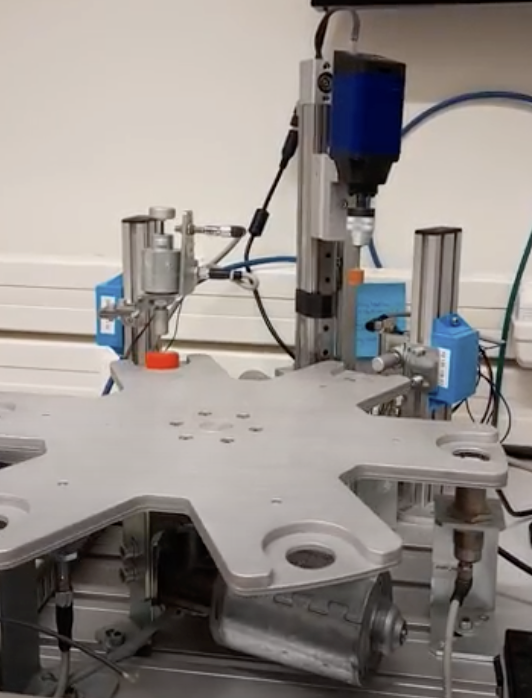
\includegraphics[scale = 0.2]{MX_Papers/Paper2/images/DT_REAL.png}
    \caption{Drilling station system.}
    \label{figure:RealImageofDrillTable}
\end{figure}

The drilling station system in Fig. \ref{figure:RealImageofDrillTable} is composed of several mechatronic components, among which, in this study we selected only the Drill and rotating Table. 
It is assumed that the mechatronic components are smart, i.e. they are equipped with their own control devices, implementing their basic operations, which are as follows. 

The Drill moves in an upward or downward direction. Whenever a workpiece is detected by the sensor under the drill, it moves downward and starts drilling. Once it completes drilling, it moves upwards and rests at the home position. 

The Table rotates from one fixed position to another. The cycle is completed when it rotates six times. 
When a workpiece is placed in the loading positions, the table rotates to bring it under the drill.

The control logic of each mechatronic component is implemented as a function block which follows the IEC 61499 standard. The function block diagram shown in Fig. \ref{figure:RealFBDiagram} consists of the two function blocks orchestrated to work together by means of event and data connections between each other and sources and sinks of sensor inputs and actuator outputs (function blocks on the left hand side and right hand side respectively). A close-up on the interacting controllers is presented in Fig. \ref{figure:RealFBControllers}.

It is assumed that the smart mechatronic components are delivered by their vendors together with the software components for implementing their control logic. They are integrated to the drilling station in a way, assuming that the control of internal operations in each mechatronic component is implemented by its predefined function block, and the integrator tries to minimise its software development effort by reusing the software components received from the vendors.
This approach requires exhaustive testing of the orchestrated system on compliance with functional and non-functional requirements. 

Hence, we will use both simulation in the loop with the plant model and formal verification in closed loop for more exhaustive exploration of the state space. 

\begin{figure}[h]
    \centering
    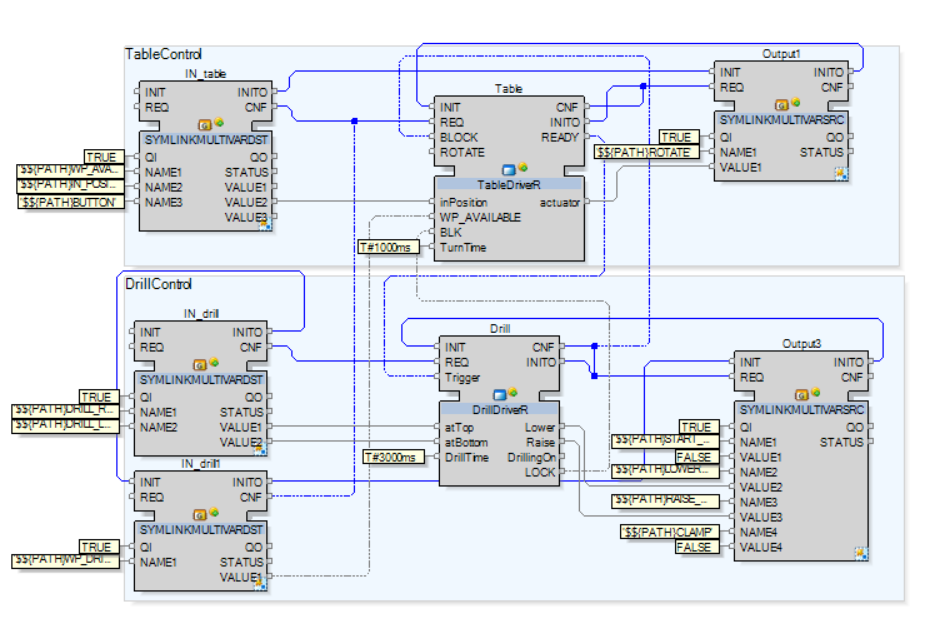
\includegraphics[scale = 0.4]{MX_Papers/Paper2/images/fig2updated.PNG}
    \caption{Function block representation of the distributed automation of drilling station.}
    \label{figure:RealFBDiagram}
\end{figure}

\begin{figure}[h]
    \centering
    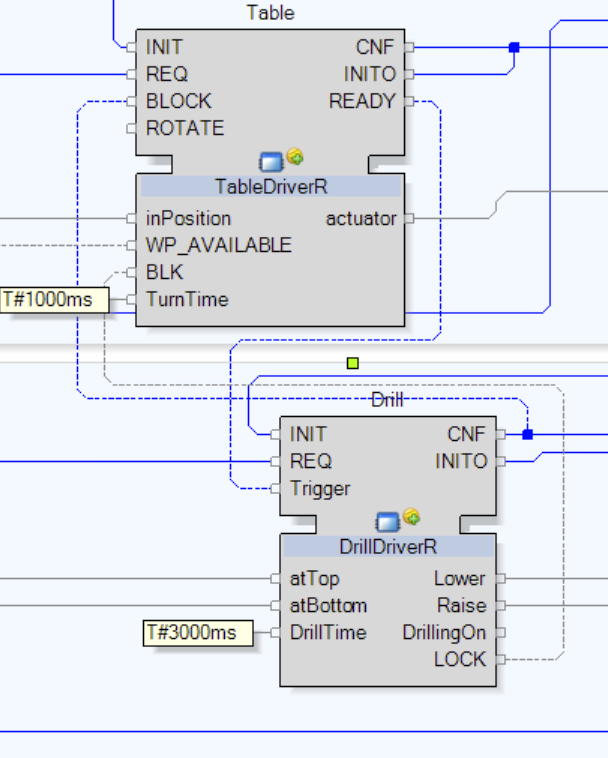
\includegraphics[scale = 0.20]{MX_Papers/Paper2/images/DT_REAL_FB_CONTROLLERS.png}
    \caption{Close-up on the decentralised controllers' interaction.}
    \label{figure:RealFBControllers}
\end{figure}

\section{Simulation Model}\label{sec:simulation_model}

The simulation-in-the-loop environment is shown in Fig. \ref{figure:SimulationFBDiagram}. The original function blocks containing the autonomous control logic of drill and table are connected with the function blocks implementing simulation models of the drill and table respectively. The controllers are also connected with each other in exactly the same way as in the real configuration in Fig. \ref{figure:RealFBControllers}. 
For example, the function block TableMod11 of type TableModTop represents a model of the table that is driven by one control signal \texttt{fwd}. When this signal receives the value \texttt{TRUE}, the simulated table starts continuous rotation clockwise. The rotation is stopped if \texttt{fwd} resets to \texttt{FALSE}.

The model outputs the Boolean value \texttt{FixPos} which becomes \texttt{TRUE} when the table comes to one of the six fixed positions. To keep the table in the fixed position, the controller has to stop motion by resetting the control signal \texttt{fwd} to \texttt{FALSE}. Besides, the model produces the \texttt{WP\_DRILL} signal, which is the reading from the sensor indicating the presence of a workpiece under the drill.

The simulation environment reproduces the working behavior of the real plant which helps to visually identify the behavior of the system before deploying the distributed control to the real hardware. Besides, the errors identified during the formal verification can be represented in simulation. 

\begin{figure}[h]
    \centering
    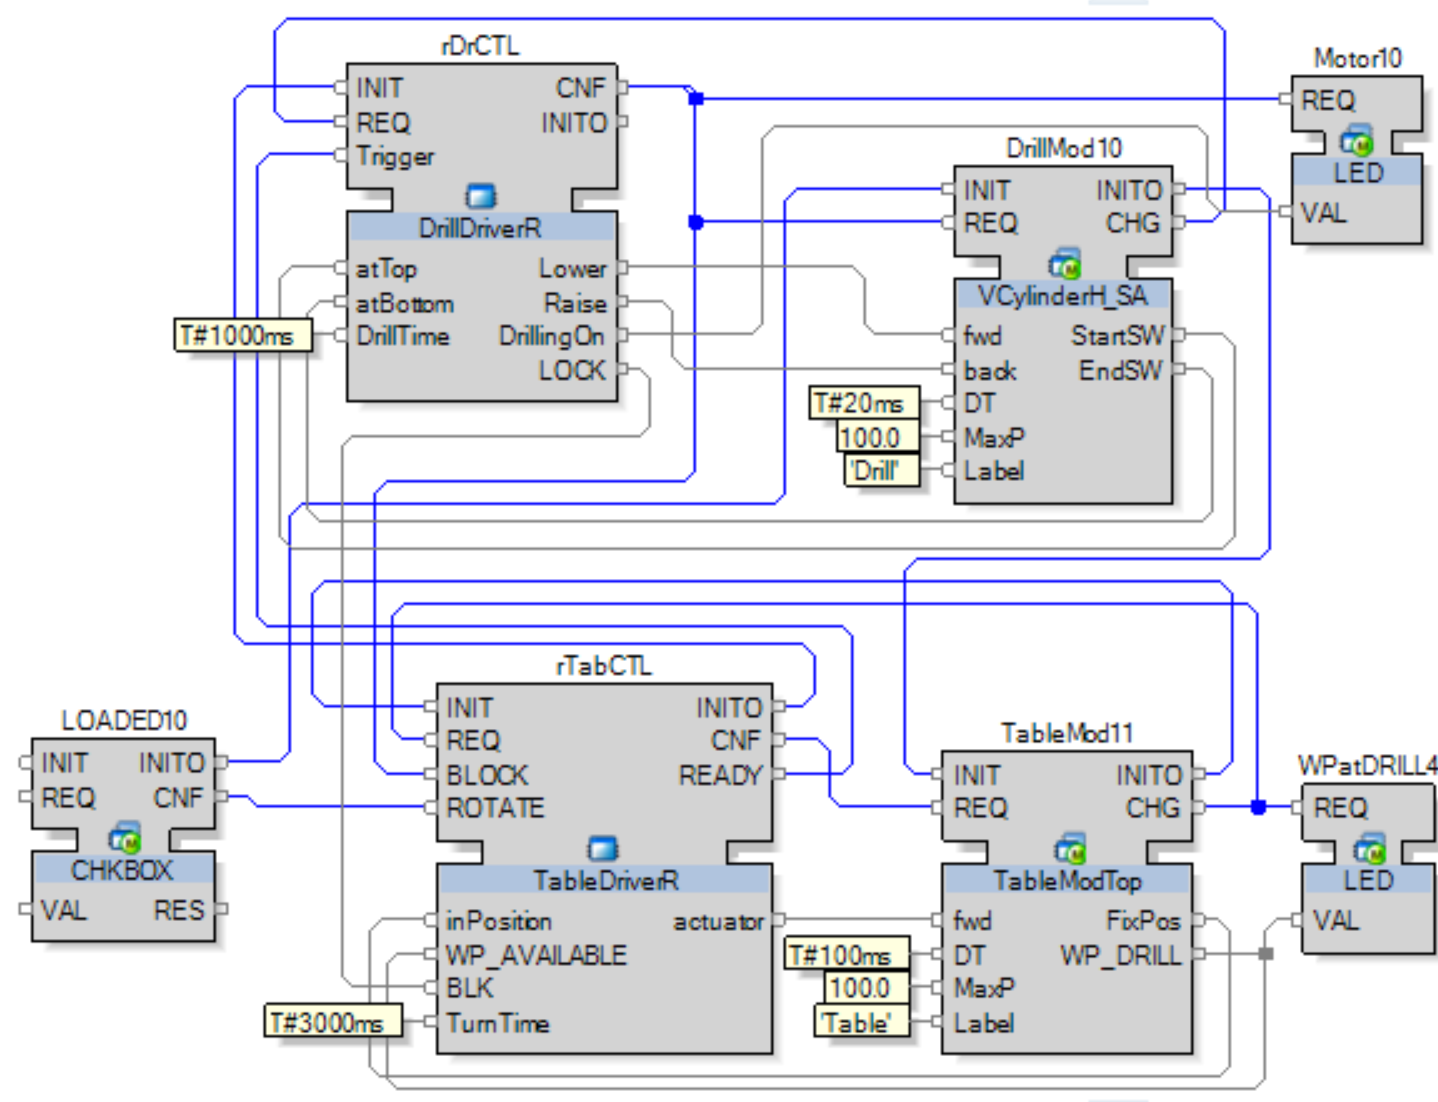
\includegraphics[scale = 0.3]{MX_Papers/Paper2/images/SimulationFBsystem.png}
    \caption{The Function Block representation of the simulation-in-the-loop configuration.}
    \label{figure:SimulationFBDiagram}
\end{figure} 

The simulation models, used in this configuration, have continuous dynamics, which is the time-domain implementation of hybrid state machine as discussed in \cite{vyatkin2008closed}. 
The core part of the plant simulation function block is based on the hybrid automaton model of the process, as illustrated in Fig. \ref{figure:Hybrid}.
The state machine has three states corresponding to the static position of the moving object, such as the vertical axis of the drill, or the rotating table. These are \texttt{stHOME}, \texttt{stEND} and \texttt{stSTOP}. There are also two dynamic states, when the coordinate of the object is changing: \texttt{dMOVETO} and \texttt{dRETURN}. 

When the state machine is in the one of the dynamic states (say, \texttt{dMOVETO}), it emits the START output event which invokes the external \texttt{E\_CYCLE} FB, which starts emitting periodic events, activating the function block with the state machine. 
The state machine remains in the \texttt{dMOVETO} state until the position reaches the end position, i.e. Pos=DIST. Until then the loopback transition condition is true, so the state-machine remains in the \texttt{dMOVETO} state. Every time the loopback transition is executed, the event CHG is emitted which also invokes the external "Integrator" FB, which recalculates the new value of the process variable based on the current value. The duration of the time interval between recalculations is determined by the \texttt{DT} parameter of the \texttt{E\_CYCLE} and speed of the motion. 

\begin{figure}[h]
    \centering
    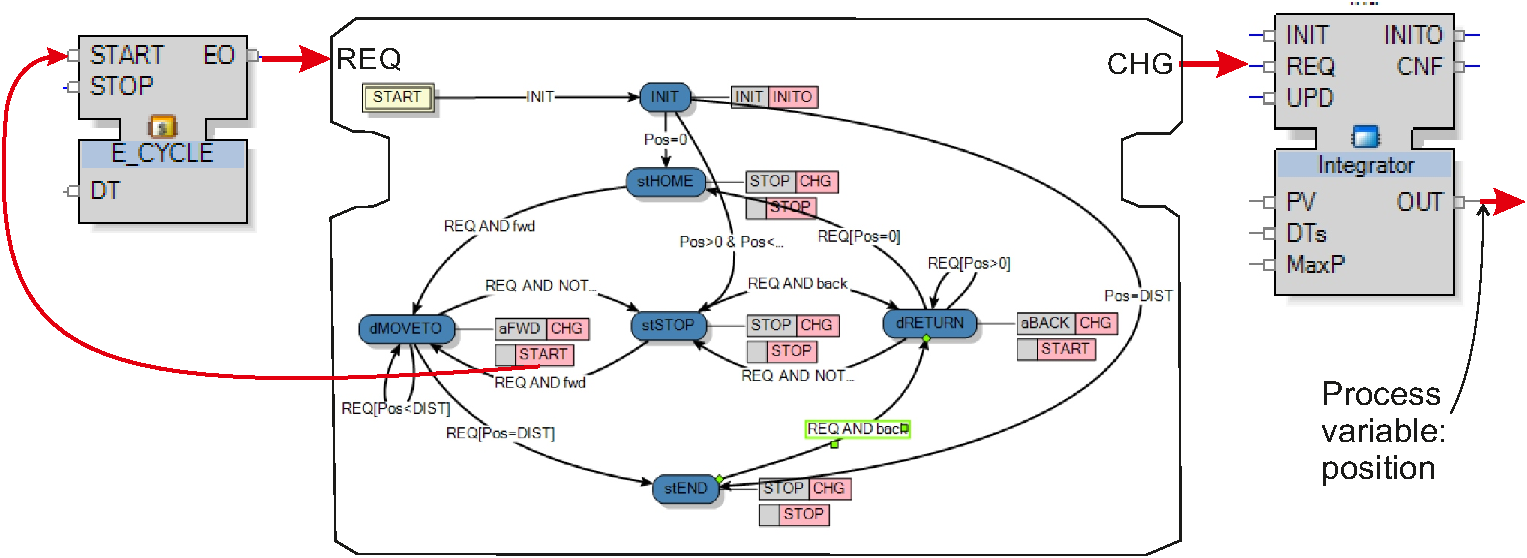
\includegraphics[scale = 0.36]{MX_Papers/Paper2/images/hybrid.pdf}
    \caption{Computational implementation of a hybrid automaton in function block.}
    \label{figure:Hybrid}
\end{figure}

Given the ever changing process values, the evolution of the model can be visually displayed using internal or external means. The development reported in this paper was done using the NxtStudio of NxtControl, which offers a proprietary visualisation technology called \texttt{CAT}. The plant model blocks were implemented as the \texttt{CATs}, therefore the model behaviour was implemented internally, within the same development environment. The interactive system visualisation by means of CATs is shown in Fig. \ref{figure:SimulationDiagram}.

\begin{figure}[h]
    \centering
    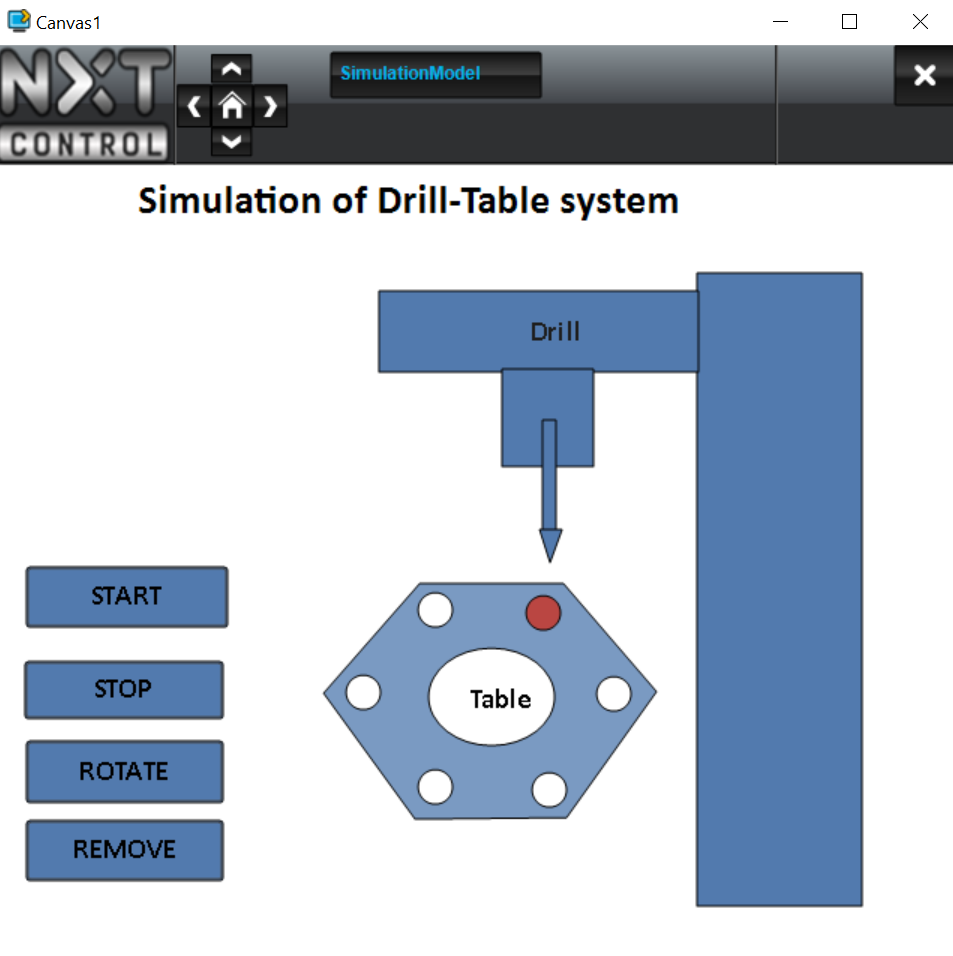
\includegraphics[scale = 0.30]{MX_Papers/Paper2/images/DT_HMI5.PNG}
    \caption{The visual representation of the simulation process.}
    \label{figure:SimulationDiagram}
\end{figure}

\section{Discrete-state Modelling Approach}\label{sec:discrete_state}

The discrete-state model of the system is created in IEC 61499 based on the simulation model described in the previous section. 

The discrete-state equivalent of the simulation configuration is shown in Fig. \ref{figure:FBver}. Here the function blocks simulating the drill and table are substituted by their analogs operating in the discrete state domain, instead of modelling the continuous process parameters, such as the drill's and table's numeric position.
The model can be then simulated in the IEC 61499 IDE with values of function block inputs and outputs displayed and modified interactively. It can be translated to the SMV model using the fb2smv tool and exposed to the formal verification by model-checking. 

\subsection{Notation for Plant Modelling}

\begin{figure}[h]
    \centering
    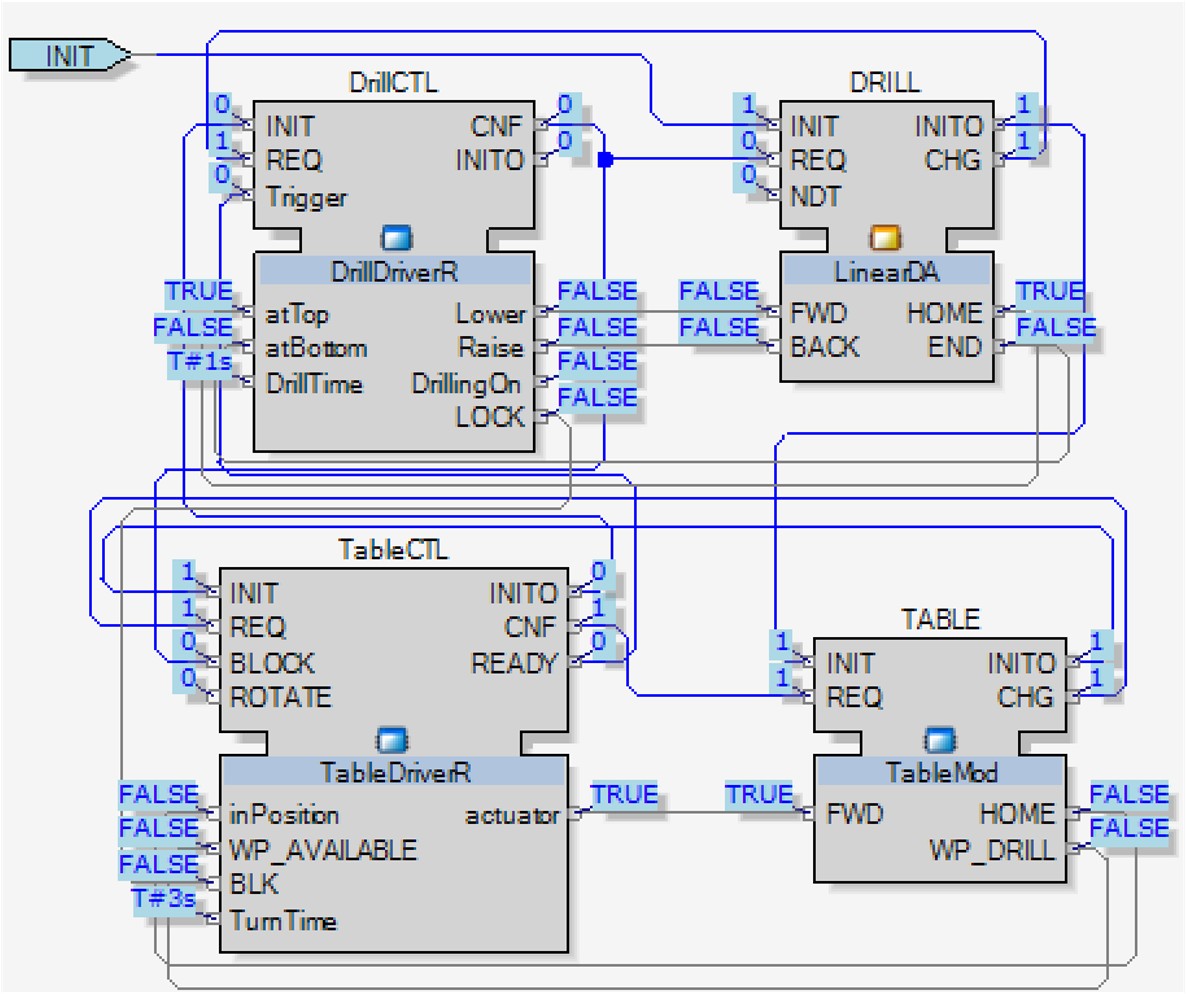
\includegraphics[scale = 0.65]{MX_Papers/Paper2/images/VerificationFB.png}
    \caption{Discrete state function block model of the Drilling station.}
    \label{figure:FBver}
\end{figure}

In the current example, the drill model is represented by an instance of a basic discrete motion model LinearDA. 
Its state-machine implementation is shown in Fig. \ref{figure:DrillECC}. The execution semantics of the state-machine follows the rules of IEC 61499, i.e. the function block is activated by an input event, and the state machine evolution is following the rules for execution control chart (ECC) of basic function blocks. 

Similarly to the hybrid state-machine in Fig. \ref{figure:Hybrid}, the discrete state model of the drill specifies three static and two dynamic states, but it does not model the position as a numeric value. The drill moves from \texttt{stHOME} to \texttt{stEND} state via a motion state called \texttt{ddMOVETO}. The state transition occurs from stHOME to ddMOVETO whenever FWD signal is TRUE. 
It is remarkable to note the NDT event input of the LinearDA function block, which remained unassigned in the application in Fig.\ref{figure:FBver}.
The NDT is reserved in the proposed modelling notation for Non-Deterministic Transition. 
Whenever the formal model generator encounters NDT in the state machine, it will interpret it accordingly. For example, the SMV modelling of NDT will be described in section \ref{sec:NDTinSMV} 

In terms of our model, the use of NDT in the transition from the motion state \texttt{ddMOVETO} to the static state \texttt{stEND} models the unknown duration of the motion from one state to another. Plant may fail whenever the \texttt{FWD} and \texttt{BACK} signals become \texttt{TRUE} simultaneously, so we introduced an ERROR state which helps to identify whether the controller creates this scenario.

\begin{figure}[h]
    \centering
    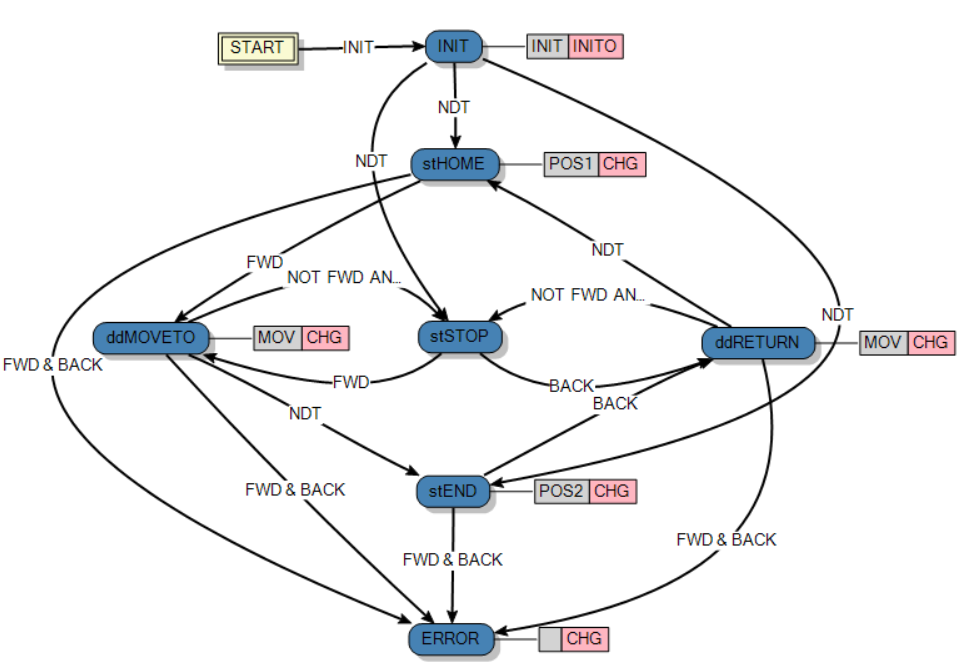
\includegraphics[scale = 0.4]{MX_Papers/Paper2/images/LinearDAFinal.PNG}
    \caption{Discrete state linear motion process model with NDT.}
    \label{figure:DrillECC}
\end{figure}

\subsection{Non Deterministic Transitions in controllers}

Non-deterministic transition can be also helpful for simplification of controller models containing timers. For example, in our case study, the controllers were developed as state machines with timeouts, therefore they are implemented in composite function blocks. In the drill, drilling process needs to be done for several durations, which is achieved with the help of The \texttt{E\_DELAY} function block. The composite function block consists of a real controller and \texttt{E\_DELAY} function block as shown in Fig. \ref{figure:DrillInterfaceControllers}(a). 

\begin{figure}[h]
    \centering
    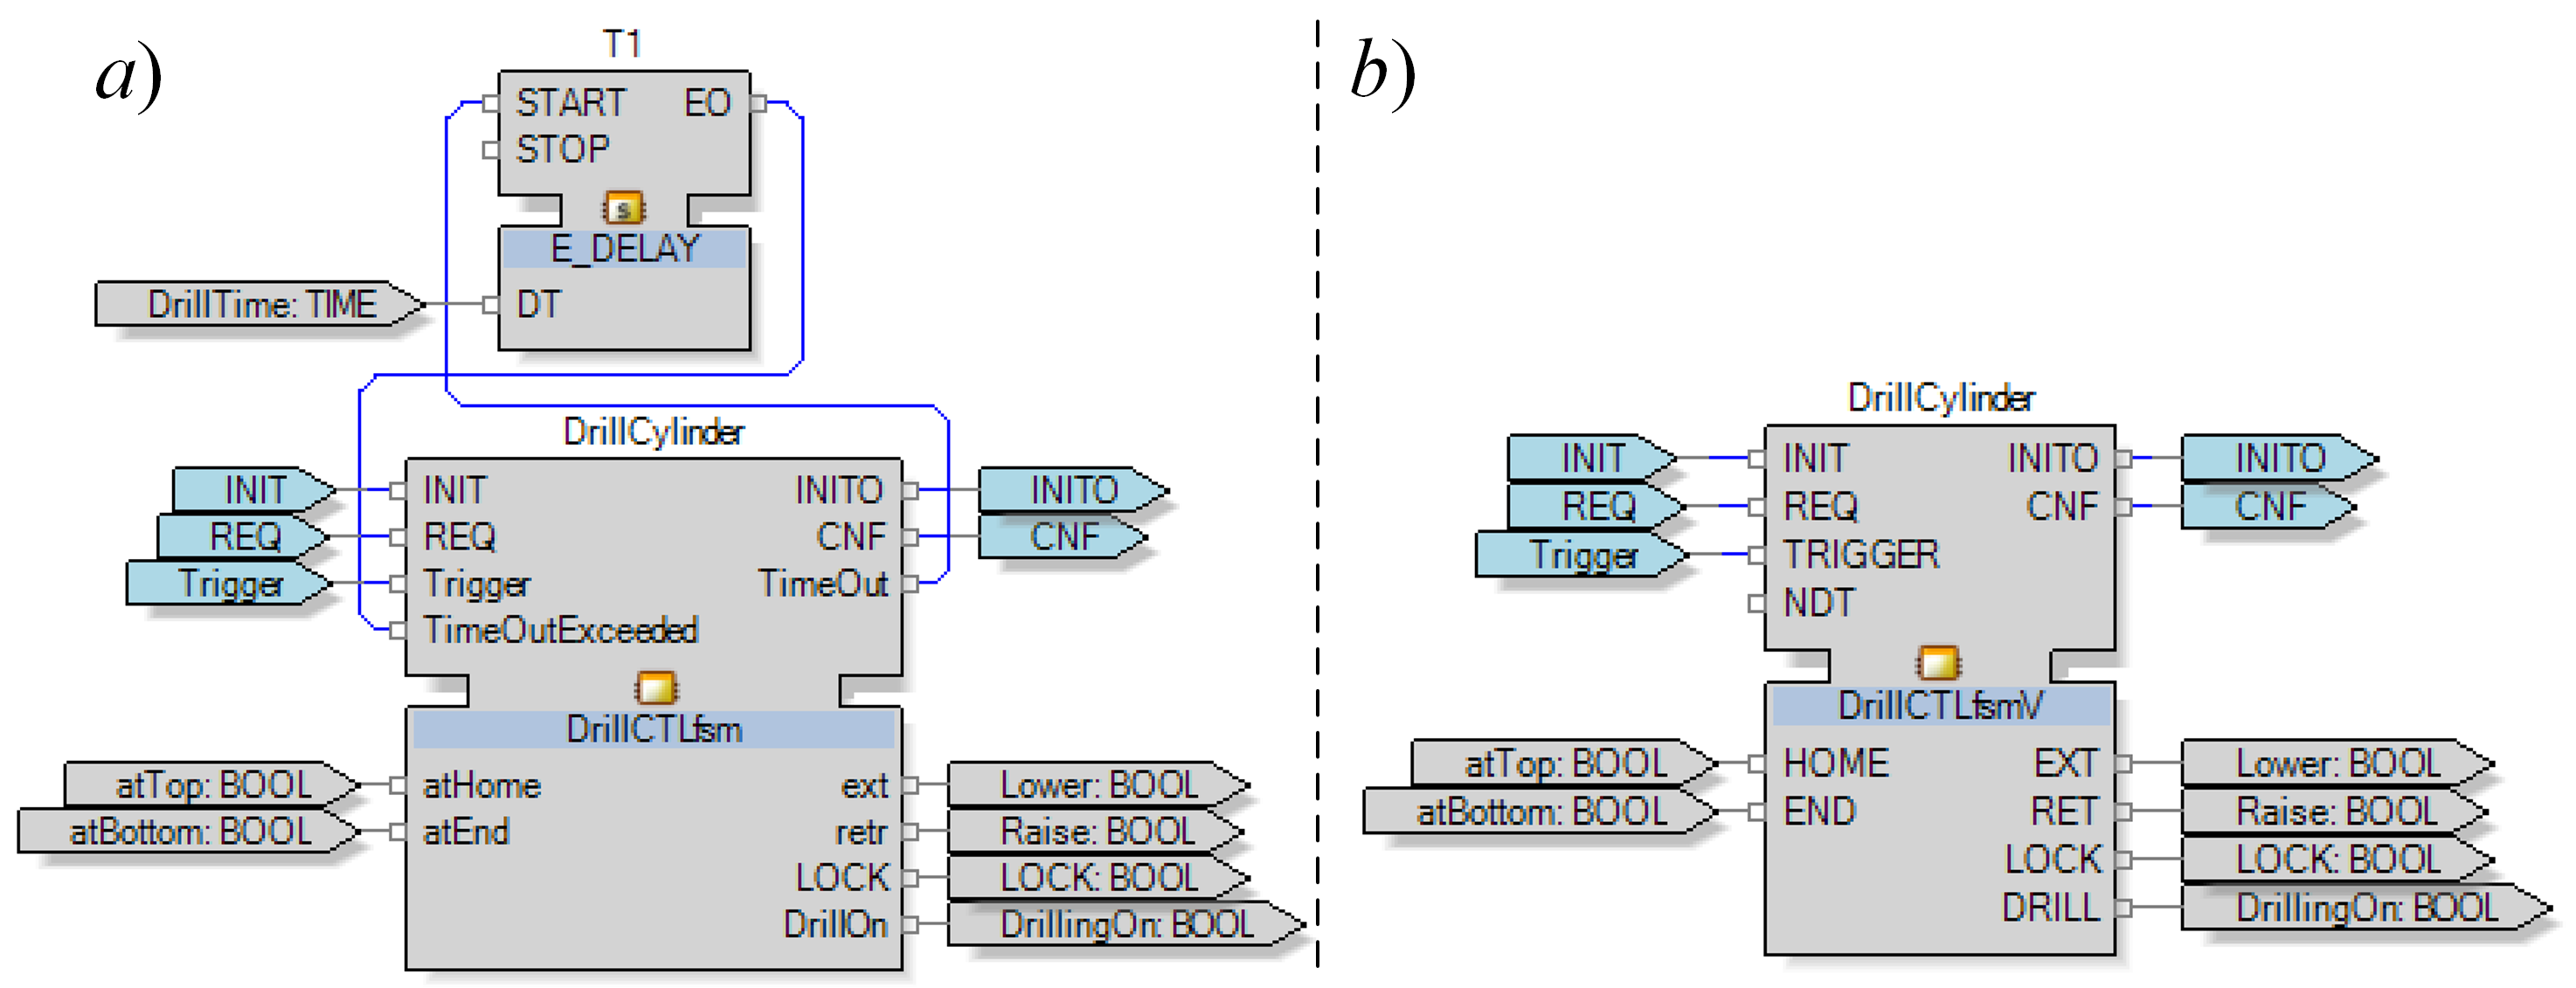
\includegraphics[scale = 0.33]{MX_Papers/Paper2/images/Fig9.png}
    \caption{a) The real drill controller with external timeout. b) The interface of modified drill Controller with non-deterministic transition input.}
    \label{figure:DrillInterfaceControllers}
\end{figure}

However, formal modelling of the timers in SMV is computationally hard. It can be avoided if the concrete delay duration was substituted by non-deterministic transitions with the help of NDT signal. Therefore, the controllers can be modified this way in order to reduce complexity of model-checking. Therefore, we removed the timeout \texttt{E\_DELAY} substituted the corresponding input of the function block and added NDT input. The execution control chart of the real drill controller and the modified drill controller are shown in Fig. \ref{figure:DrillECCControllers}.

\begin{figure}[h]
    \centering
    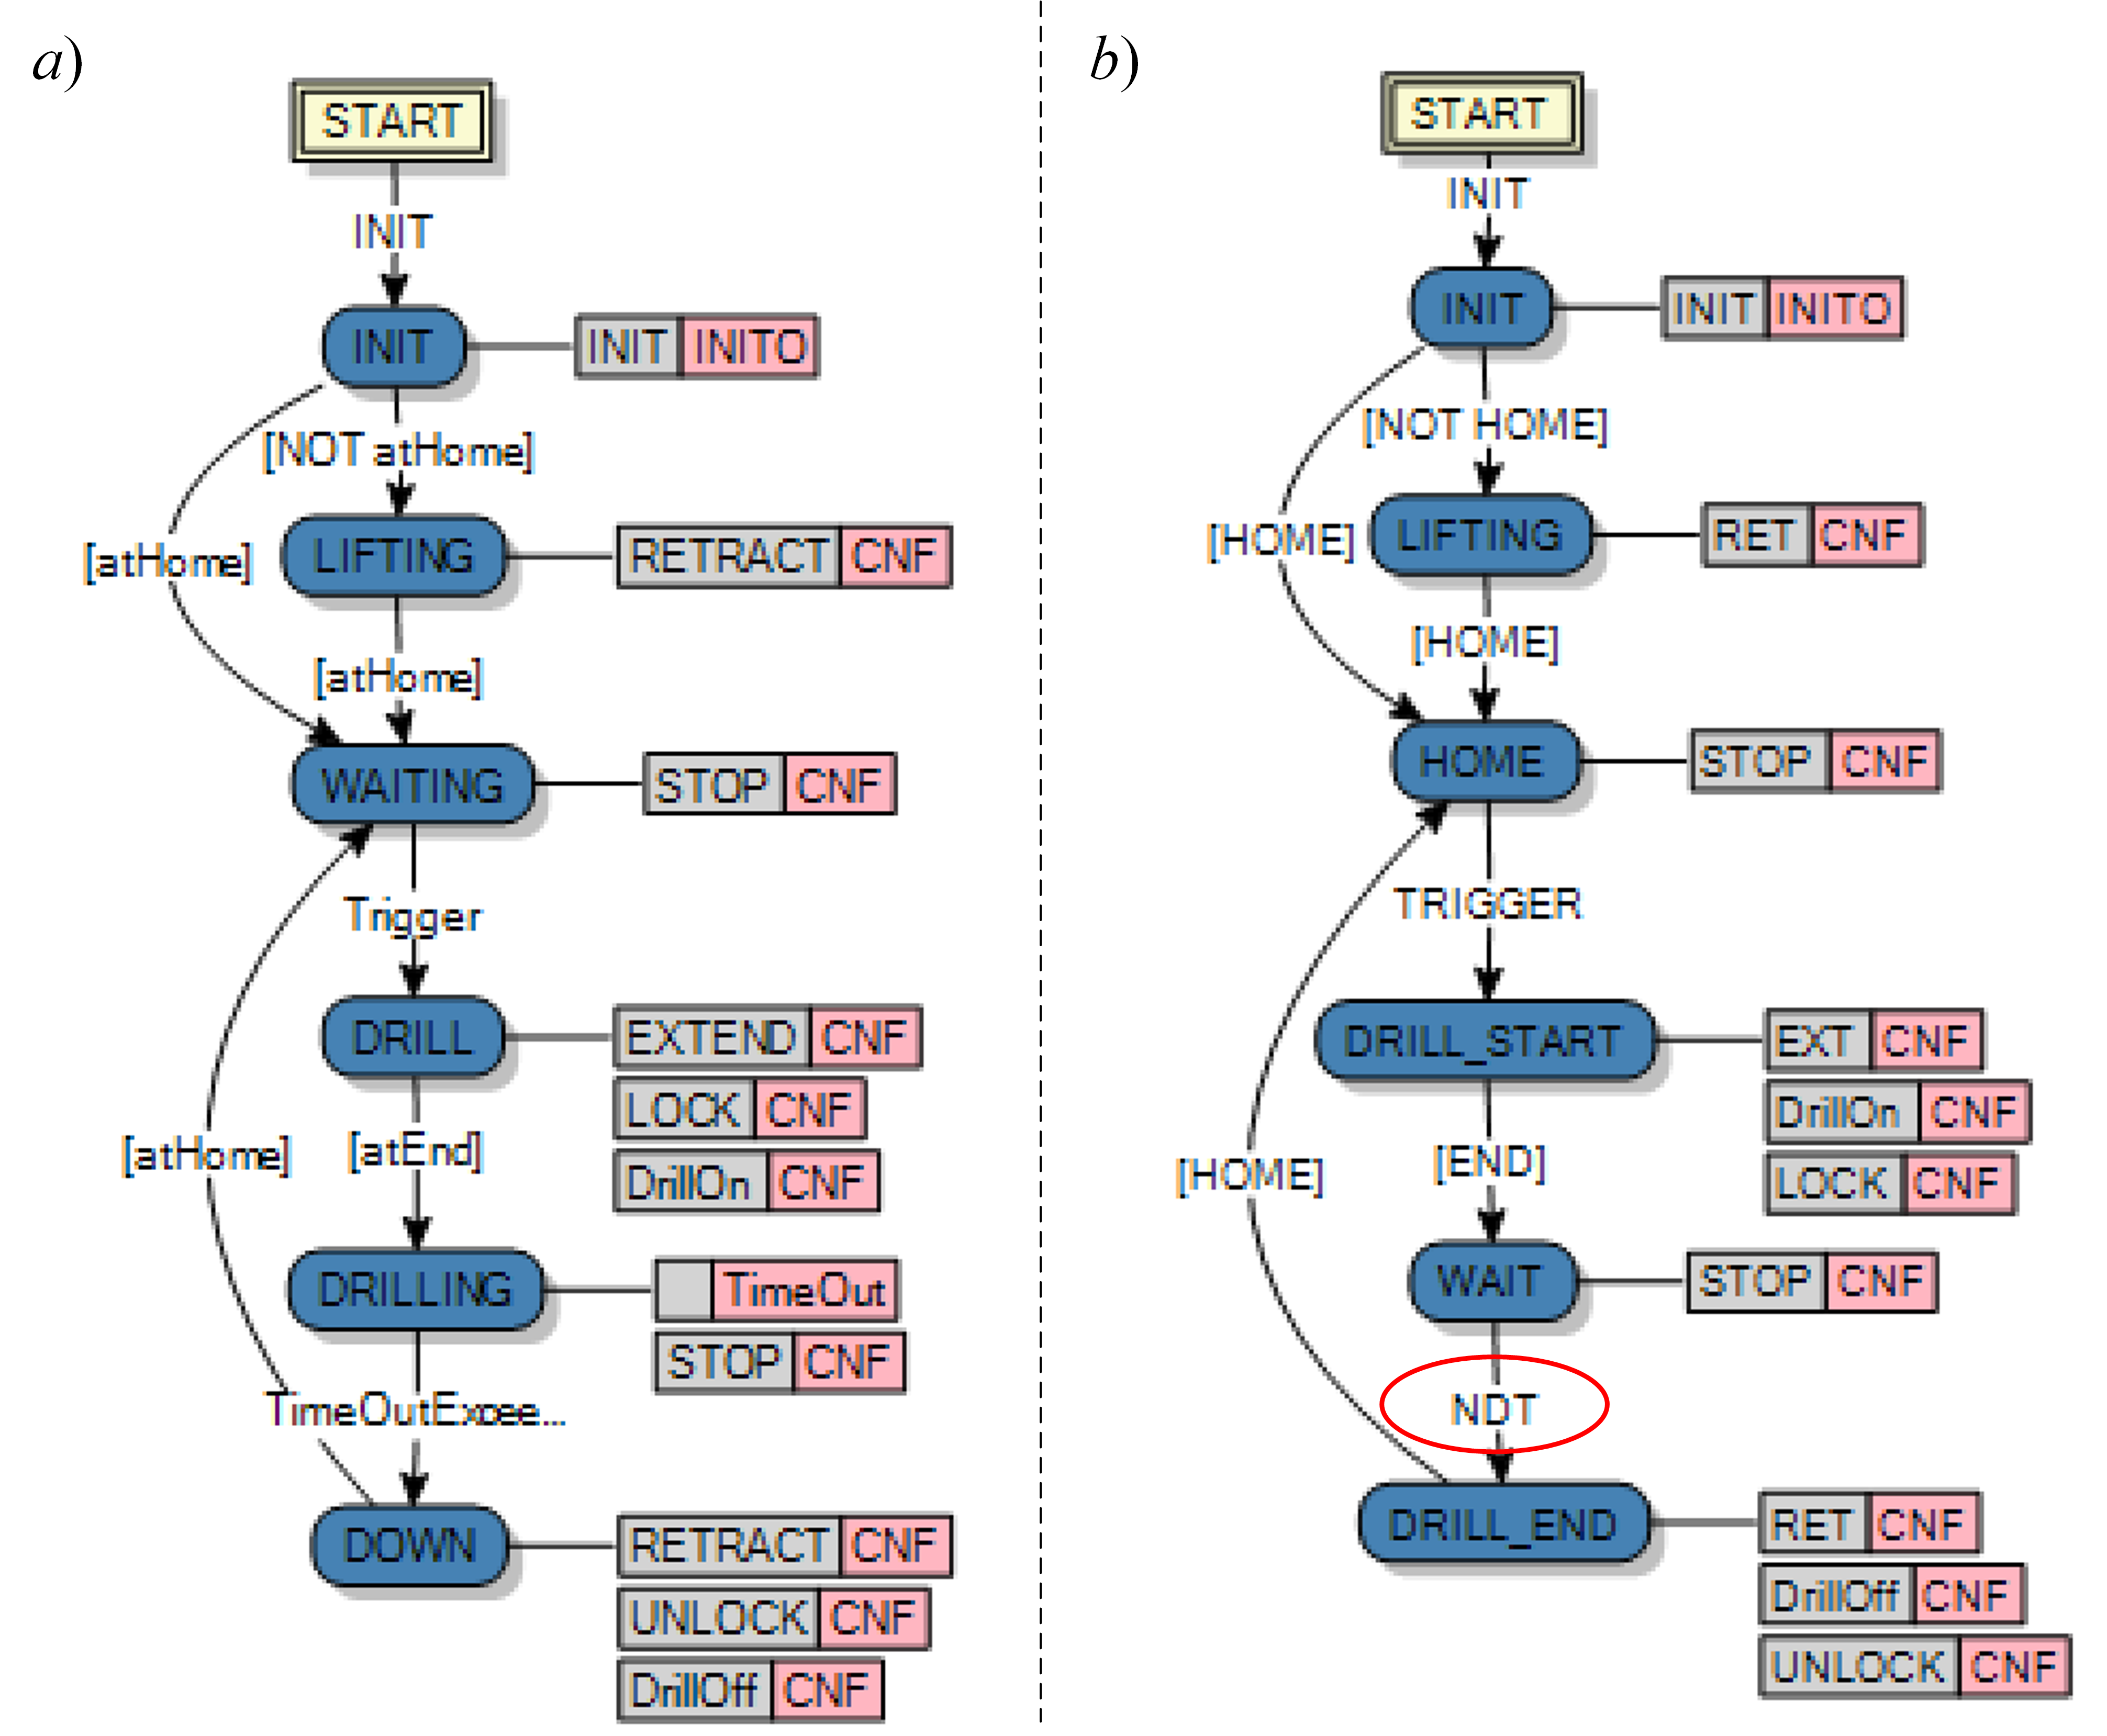
\includegraphics[scale = 0.24]{MX_Papers/Paper2/images/Fig10.png}
    \caption{a) The ECC of the real drill controller; b) The ECC of the modified drill controller with a non-deterministic transition modelling the time delay.}
    \label{figure:DrillECCControllers}
\end{figure}

\subsection{Modelling of non-determinism in SMV}\label{sec:NDTinSMV}

SMV provides a way to accomplish non-deterministic choice by providing a set of values to the signal. The first statement is used to declare the variable NDT as a Boolean type and the second statement is used to initialize the NDT variable to either TRUE or FALSE value.

\begin{lstlisting}[breaklines,basicstyle=\small]
1 | VAR NDT:= boolean;
2 | init(NDT):= { TRUE, FALSE };
\end{lstlisting}

In every transition we are giving a provision to choose either TRUE or FALSE. This makes the NDT variable unpredictable in each transition.

\begin{lstlisting}[breaklines,basicstyle=\small]
3 | next(NDT):={ TRUE, FALSE };
\end{lstlisting}

Implementing non-determinism in every transition can be limited by introducing conditions in the next statement. If it is not required for the NDT variable to choose values in every transition then we can design like below:

\begin{lstlisting}[breaklines,basicstyle=\small]
4 | next(NDT):= case
5 | 	Condition: { TRUE, FALSE };
6 |     TRUE : NDT;
7 | Esac;
\end{lstlisting}

\section{fb2smv tool}\label{sec:fb2smv_tool}

The \textbf{fb2smv} tool \cite{fb2smv} is a model generator for generating SMV models of function block systems in IEC 61499. It is a part of formal verification tool-chain, that includes the model checker NuSMV and the tool for counterexample analysis in terms of the original FB system. 

The tool implements the formal model of IEC 61499 as per the modelling method present in \cite{drozdov2021formal}. In order to construct \texttt{SMV} code, the \textbf{fb2smv} tool uses Abstract State Machine (ASM) \cite{gurevich1995evolving} as an intermediate model. The tool takes IEC 61499 function blocks expressed in XML format as input and generates a formal model with the help of ASM semantics. According to \cite{drozdov2021formal}, the structure of \texttt{SMV} code consists of the declaration part and the rules part, which are the ASM rules.

The tool converts basic and composite function blocks and also includes more additional features like, limiting the boundaries of variables to reduce the state space, changing execution order of FBs, deciding the input event priority by changing its order etc. The proposed non-deterministic transitions notation has been added to the tool as a result of this work. 

\section{Results and Analysis}\label{sec:results}

In this paper, we demonstrated on a case study example, the use of IEC 61499 language for design and formal verification of cyber-physical automation systems. First, we designed the control logic of each mechatronic component in a drilling station and then implemented it as a function block in IEC 61499 standard. The simulation environment of the drilling station is developed with the help of the same controllers which are used in the real configuration. We reproduced the same plant behavior in the simulation model using the function blocks. In order to create a formal model of the system, we transformed existing function blocks of the plant models and controllers by adding non-deterministic transitions, using the proposed NDT notation. Using fb2smv we converted the functional blocks to SMV code, which was verified using NuSMV on a machine with Intel(R) core(TM) i7-10510U CPU @1.80GHz 2.30GHz with 32GB RAM. The simulate feature of NuSMV was used to check the formal model's working behavior. Simulating the SMV code in interactive mode gives us the provision to go through each state by giving appropriate sensor inputs. We can try all possible input combinations to verify whether the system behaves as we expected. We can also randomly simulate the traces or we can manually go through each state by selecting different input combinations.

The main drawback of simulation is that the number of possible behaviors can be too large or even infinite. Simulation can show the presence of bugs, not their absence. 

More comprehensive verification can also be done by model-checking various properties, i.e. checking whether a requirement is true or not in all possible execution traces of control logic. This will allow us to test critical scenarios where there can be failures in some combination of inputs. The formal model of the system was verified with help of CTL \cite{emerson1985decision} specifications. While testing the CTL specifications in NuSMV, we found the following statement is false so it is possible that the table can rotate while the drilling process is going on.

\begin{lstlisting}[breaklines,basicstyle=\small]
-- specification  G !(DRILL_TABLE_CFB3_inst.DrillCTL_RET = TRUE & DRILL_TABLE_CFB3_inst.ActuatorGen_EO = TRUE)  
\end{lstlisting}

While executing the above specification, the NuSmv gave a counterexample that contradicts this statement. The counterexample generation for the above specification took 26000 seconds to complete. The counterexample helps to identify the error in the controller's design. We tested the same logic in the simulation model, the table rotated from its current position to another while drilling the workpiece. The real system also exhibits the same issue.

To fix this issue we need to analyze the counterexample provided by the NuSMV, but identifying the variables changed in each iteration is difficult. The Nutrac tool provides a better way to understand each state. The Nutrac tool converts the counterexample to a CSV file. This CSV file's columns represent states and rows represent input/output events or data input/output variables. We analyzed the CSV file and identified the issue. The issue was present in the execution control chart of the table's controller. It is required to add the BLOCK signal and it should be checked before moving from DRILLED state to REMOVED state. We verified the CTL specification again and this time NuSMV gave the TRUE result. The modified controller is tested in the real object, as well as in a simulation system and it was behaving as we expected i.e table was not able to rotate while drilling is going on.

In order to identify whether the controller produces the \texttt{FWD} and \texttt{BACK} signals true at the same time, the following specification is used.

\begin{lstlisting}[breaklines,basicstyle=\small]
-- specification  G !(DRILL_TABLE_CFB3_inst.DRILL.Q_smv = ERROR_ecc)
\end{lstlisting}

After executing the above specification, the NuSMV produced the output as TRUE. The ECC of the drill model never goes to ERROR\_ecc state i.e. the controller never produces \texttt{FWD=TRUE} and \texttt{BACK=TRUE} condition simultaneously.  

This paper \cite{vyatkin2003verification} proposes a software tool called VEDA (verification environment for distributed application), which is used for closed loop modelling and verification of distributed control systems in intelligent manufacturing. Manually developed plants and automatically generated controllers are combined for model-based verification in IEC 61499 standard but it requires higher integration effort. The paper \cite{Time-AwareComputations1} \cite{Time-AwareComputations2} describes a closed loop system with a simulation model used to autogenerate SMV but the resulting complexity was prohibitive. In this paper, we propose a methodology to create a closed-loop model staying within IEC 61499 standard which produces lower complexity of model-checking than \cite{Time-AwareComputations1} \cite{Time-AwareComputations2} and reasonable engineering effort that is less than in \cite{vyatkin2003verification}.  

\section{Conclusion and Future Work}\label{sec:conclusion}

In this paper, we proposed a tool chain which helps to verify and analyze the function blocks implemented in IEC 61499 standard. This tool chain can be used for continuous development and evaluation of distributed control systems. With the help of this tool chain, it is possible to test the system quickly and efficiently. The accurate implementation formal model is necessary to identify all possible flaws in the system. The existing functionalities of fb2smv along with the non-deterministic transitions in function blocks help to provide a similar formal model of the system. Previously, the counterexample analysis was complicated but now the Nutrac tool solves this issue by giving a better representation of counterexample in CSV format. The developers working on complex system design can use this tool chain for continuous development and testing.

The non-deterministic transitions in function blocks can be extended by introducing NDT as a variable to the FBs. This NDT variable can be any of any IEC 61499 data type but the NDT variable should be able to choose one value from set values. For example, if we introduce NDT as a variable of integer data type and its values limited 0 to 5 then it should be able to randomly select one value from 0 to 5. In order to introduce more randomness to our formal model, it's better to implement NDT as a variable instead of using NDT as an event signal. An interesting field to explore is if we can generate the specification as well as the plant model automatically then existing manual interventions can be avoided. The tool chain which identifies all possible errors and fixes them automatically could be the next step in the future.

The models used in this paper are not based on time so the timing problems due to different set of time scales of controller and plant cannot be identified by this approach. The extension of notation to timed automata can be added for future work.

\section{Acknowledgements}
This work was sponsored, in part, by the H2020 project 1-SWARM co-funded by the European Commission (grant agreement: 871743).  

%%% Put references here
\putbib
\end{bibunit}
